\documentclass[aspectratio=169]{beamer}

\usepackage[utf8]{inputenc}
\usepackage[english]{babel}
\usepackage[T1]{fontenc}
\usepackage{lmodern}
\usepackage{bbm}
\usepackage{listings}
\usepackage{multicol}
\usepackage{csquotes}
\usepackage{hyperref}
\usepackage{indentfirst}
\usepackage{amsthm}
\usepackage{amsfonts}
\usepackage{amsmath}
\usepackage{amssymb}
\usepackage{mathtools}
\usepackage{tikz}
\usepackage{xcolor}
\usepackage{array}
\usepackage{booktabs}

\newcommand{\id}[1]{\ensuremath{\mathit{#1}}}
\newcommand{\kw}[1]{\ensuremath{\mathtt{#1}}}
\newcommand{\Let}{\kw{let}}
\newcommand{\In}{\kw{in}}
\newcommand{\If}{\kw{if}}
\newcommand{\Then}{\kw{then}}
\newcommand{\Else}{\kw{else}}
\newcommand{\Filter}{\kw{filter}}
\newcommand{\Or}{\kw{or}}
\newcommand{\Groupby}{\kw{groupby}}
\newcommand{\Partition}{\kw{partition}}
\newcommand{\Scatter}{\kw{scatter}}
\newcommand{\Hist}{\kw{hist}}
\newcommand{\Map}{\kw{map}}
\newcommand{\Sum}{\kw{sum}}
\newcommand{\Mod}{\kw{mod}}
\newcommand{\Fst}{\kw{fst}}
\newcommand{\Snd}{\kw{snd}}
\newcommand{\Presum}{\kw{presum}}
\newcommand{\True}{\kw{true}}
\newcommand{\False}{\kw{false}}
\newcommand{\Sort}{\kw{sort}}
\newcommand{\Segor}{\kw{segor}}
\newcommand{\Hash}{\kw{hash}}
\newcommand{\Random}{\kw{random}}
\newcommand{\Iota}{\kw{iota}}
\newcommand{\Unzip}{\kw{unzip}}
\newcommand{\Unit}{\mathbf{unit}}
\newcommand{\Int}{\mathbf{int}}
\newcommand{\Bool}{\mathbf{bool}}
\newcommand{\Def}{\kw{def}}
\newcommand{\Rep}{\kw{rep}}
\newcommand{\Zip}{\kw{zip}}

\usetikzlibrary{automata, positioning, arrows}

\graphicspath{ {./figures/} }

\definecolor{palepurple}{rgb}{0.7647,0.69411,0.88235}
\definecolor{palepurple}{rgb}{0.7647,0.69411,0.88235}
\definecolor{midviolet}{rgb}{0.6,0.4,0.8}

\newcolumntype{M}[2]{>{\centering\arraybackslash}m{#1}<{\rule{0pt}{#2}}}
\newcommand{\darkpalepurple}{palepurple!70!black}
\definecolor{paleyellow}{rgb}{1.0,1.0,0.7725}
\setbeamercolor{background canvas}{bg=paleyellow}

\usetheme{default}
\usecolortheme{wolverine}
\setbeamercolor*{palette primary}{bg=palepurple}
\setbeamercolor*{palette quaternary}{bg=palepurple}
\setbeamercolor{structure}{fg=palepurple}
\setbeamertemplate{navigation symbols}{\insertframenumber/\inserttotalframenumber}
\setbeamertemplate{blocks}[rounded][shadow]
\setbeamercolor{frametitle}{bg=midviolet,fg=black}
\setbeamercolor{block title}{bg=structure, fg=black}
\setbeamercolor{block body}{bg=structure, fg=black}
\setbeamercolor{block title alerted}{bg=structure, fg=black}
\setbeamercolor{block body alerted}{bg=structure, fg=black}
\setbeamercolor{block title example}{bg=structure, fg=black}
\setbeamercolor{block body example}{bg=structure, fg=black}
\setbeamercolor{frametitle}{bg=palepurple,fg=black}


\setbeamertemplate{itemize item}{\scriptsize$\blacksquare$}
\setbeamertemplate{itemize subitem}{\scriptsize$\blacksquare$}
\setbeamertemplate{itemize subsubitem}{\scriptsize$\blacksquare$}

\title[Hash Maps]{Functional Hash Maps in a Data Parallel Language}
\author{\textbf{William Henrich Due} \inst{1} \and Martin Elsman \inst{1} \and Troels Henriksen \inst{1}}
\institute[shortinst]{\inst{1} Department of Computer Science, University of Copenhagen}
\date{August 22nd, 2025}

\begin{document}

\begin{frame}
  \begin{center}
    \titlepage
    \vfill
    \usebeamerfont{institute} Contact: \url{widu@di.ku.dk}
  \end{center}
\end{frame}

\begin{frame}\frametitle{Open Adressing Example}
  \begin{columns}
  \begin{column}{.48\textwidth}
  \hfill
  \begin{itemize}
    \item Keys $k_0, k_1 \in K$.
    \item Hash function $h: K \to \{0, 1, 2, 3\}$.
    \item $h(k_0) = h(k_1) = 1$.
  \end{itemize}
  \hfill  
  \end{column}
  \hfill
  \begin{column}{.5\textwidth}
    $$
    \begin{array}{|M{1cm}{0.4cm}|M{1cm}{0.4cm}|M{1cm}{0.4cm}|M{1cm}{0.4cm}|}
      \hline
      & \only<2,4->{$k_0$} \only<3>{$k_0, \color{red}{k_1}$} & \only<4->{$k_1$} & \\ \hline
    \end{array}
    $$
  \end{column}
  \end{columns}
\end{frame}

\begin{frame}\frametitle{Core Ideas}
  \begin{columns}
  \begin{column}{.38\textwidth}
  \hfill
  \begin{itemize}
    \item<1-> Concurrency.
    \item<2-> Collision resolution.
    \item<3-> Functional Array Languages.
  \end{itemize}
  \hfill  
  \end{column}
  \hfill
  \begin{column}{.6\textwidth}
    \onslide<2->{
       $$
    \begin{array}{|M{1cm}{0.4cm}|M{1cm}{0.4cm}|M{1cm}{0.4cm}|M{1cm}{0.4cm}|}
      \hline
      & $k_0$ & $k_1$ & \\ \hline
    \end{array}
    $$
    \begin{center}
      or
    \end{center}
    $$
    \begin{array}{|M{1cm}{0.4cm}|M{1cm}{0.4cm}|M{1cm}{0.4cm}|M{1cm}{0.4cm}|}
      \hline
      & $k_1$ & $k_0$ & \\ \hline
    \end{array}
    $$
    }
    \onslide<3->{
      \begin{align*}
        \Map & : (\alpha \to \beta) \to [n]\alpha \to [n]\beta
      \end{align*}  
    }
  \end{column}
  \end{columns}
\end{frame}
\begin{frame}\frametitle{Perfect Hashing with FKS}
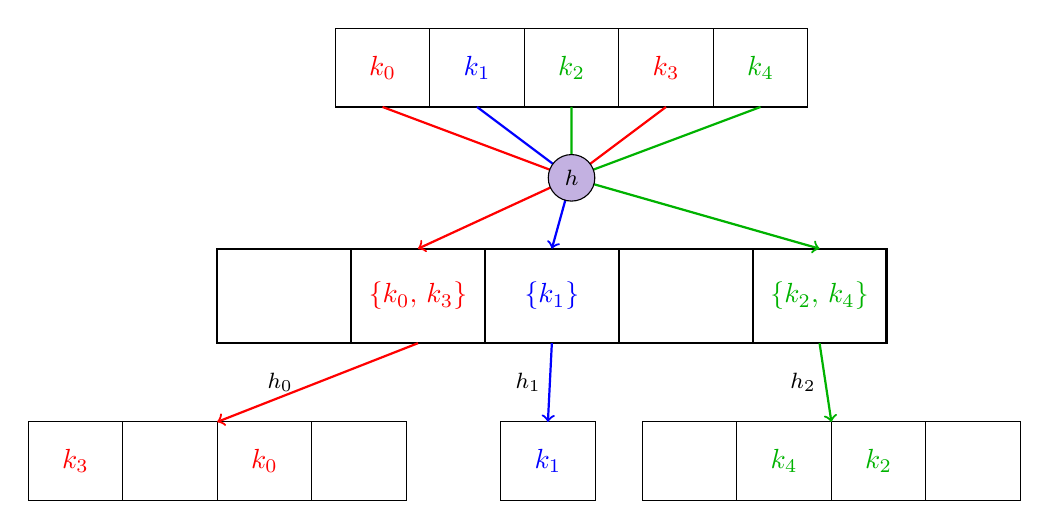
\begin{tikzpicture}

% Vertical positions
\def\yTop{3.0}
\def\yMid{0.0}
\def\yarrays{-1}

% Horizontal positions for arrays
\def\xA{0}          % First 4-cell array (left)
\def\xB{6}          % Single cell array (middle)
\def\xC{7.8}        % Second 4-cell array (right)

% Wider cells for hash buckets
\def\cellW{1.7}
\def\cellH{1.2}

% Center the middle array relative to the bottom arrays
\def\xMid{2.4}      % Centered position for middle array
\def\xTop{3.9}      % Keep top array position for keys

\foreach \i in {0,...,4} {
  \draw (\xTop+\i*1.2,\yTop) rectangle (\xTop+\i*1.2+1.2,\yTop+1);
  % Color k_0 and k_3 red, k_1 blue, k_2 and k_4 green
  \ifnum\i=0
    \node[text=red] at (\xTop+\i*1.2+0.6,\yTop+0.5) {$k_{0}$};
  \else\ifnum\i=3
    \node[text=red] at (\xTop+\i*1.2+0.6,\yTop+0.5) {$k_{3}$};
  \else\ifnum\i=1
    \node[text=blue] at (\xTop+\i*1.2+0.6,\yTop+0.5) {$k_{1}$};
  \else\ifnum\i=2
    \node[text=green!70!black] at (\xTop+\i*1.2+0.6,\yTop+0.5) {$k_{2}$};
  \else\ifnum\i=4
    \node[text=green!70!black] at (\xTop+\i*1.2+0.6,\yTop+0.5) {$k_{4}$};
  \else
    \node at (\xTop+\i*1.2+0.6,\yTop+0.5) {$k_{\i}$};
  \fi\fi\fi\fi\fi
}

% Middle array: 5 bigger cells for "bins", only some filled with sets
\foreach \i in {0,...,4} {
  \draw[thick] (\xMid+\i*\cellW,\yMid) rectangle (\xMid+\i*\cellW+\cellW,\yMid+\cellH);
}
% Only fill h_1, h_2, h_4
\node[text=red] at (\xMid+1*\cellW+0.5*\cellW,\yMid+0.6) {$\{k_{0},\,k_{3}\}$};
\node[text=blue] at (\xMid+2*\cellW+0.5*\cellW,\yMid+0.6) {$\{k_{1}\}$};
\node[text=green!70!black] at (\xMid+4*\cellW+0.5*\cellW,\yMid+0.6) {$\{k_{2},\,k_{4}\}$};

% Optional bin labels (smaller, not highlighted)
\foreach \i in {0,...,4} {
  \node[font=\scriptsize] at (\xMid+\i*\cellW+0.5*\cellW,\yMid-0.25) {};
}

% Bottom arrays (unchanged)
% First array of 4 simple boxes (left)
\foreach \j in {0,...,3} {
  \draw (\xA+\j*1.2,\yarrays) rectangle (\xA+\j*1.2+1.2,\yarrays-1);
}
\node[text=red] at (\xA+0.6,\yarrays-0.5) {$k_3$}; % first cell
\node[text=red] at (\xA+3.0,\yarrays-0.5) {$k_0$}; % fourth cell

% Single box array (middle)
\draw (\xB,\yarrays) rectangle (\xB+1.2,\yarrays-1);
\node[text=blue] at (\xB+0.6,\yarrays-0.5) {$k_1$}; % middle box

% Second array of 4 simple boxes (right)
\foreach \j in {0,...,3} {
  \draw (\xC+\j*1.2,\yarrays) rectangle (\xC+\j*1.2+1.2,\yarrays-1);
}
\node[text=green!70!black] at (\xC+1.8,\yarrays-0.5) {$k_4$}; % second cell
\node[text=green!70!black] at (\xC+3.0,\yarrays-0.5) {$k_2$}; % fourth cell

% Arrows from topmost k_i to bins - First show all keys going to h
% All keys point to a central h point
\def\hPoint{(\xTop+2.5*1.2,\yTop-0.9)}

% Lines from each key to the central h point
\draw[->, thick, red] (\xTop+0.6,\yTop) -- \hPoint;
\draw[->, thick, red] (\xTop+3*1.2+0.6,\yTop) -- \hPoint;
\draw[->, thick, blue] (\xTop+1*1.2+0.6,\yTop) -- \hPoint;
\draw[->, thick, green!70!black] (\xTop+2*1.2+0.6,\yTop) -- \hPoint;
\draw[->, thick, green!70!black] (\xTop+4*1.2+0.6,\yTop) -- \hPoint;

% Arrows from h to each bin
\draw[->, thick, red] \hPoint -- (\xMid+1*\cellW+0.5*\cellW,\yMid+\cellH);
\draw[->, thick, blue] \hPoint -- (\xMid+2*\cellW+0.5*\cellW,\yMid+\cellH);
\draw[->, thick, green!70!black] \hPoint -- (\xMid+4*\cellW+0.5*\cellW,\yMid+\cellH);

% Label the hash function h at the central point
\node[font=\footnotesize, circle, draw, fill=palepurple] at \hPoint {$h$};

% Arrows: h_1, h_2, h_4 to bottom arrays (h_1 arrow RED, h_2 arrow BLUE, h_4 arrow GREEN)
\draw[->, thick, red] (\xMid+1*\cellW+0.5*\cellW,\yMid) -- (\xA+2.4,\yarrays); % h1 to center of left 4-cell array
\node[font=\footnotesize] at (\xMid+1*\cellW-0.9,\yMid-0.5) {$h_0$};

\draw[->, thick, blue] (\xMid+2*\cellW+0.5*\cellW,\yMid) -- (\xB+0.6,\yarrays); % h2 to center of 1-cell array
\node[font=\footnotesize] at (\xMid+2*\cellW+0.5*\cellW-0.3,\yMid-0.5) {$h_1$};

\draw[->, thick, green!70!black] (\xMid+4*\cellW+0.5*\cellW,\yMid) -- (\xC+2.4,\yarrays); % h4 to center of right 4-cell array
\node[font=\footnotesize] at (\xMid+4*\cellW+0.2*\cellW+0.3,\yMid-0.5) {$h_2$};

\end{tikzpicture}
\end{frame}

\begin{frame}\frametitle{Finding collision-free hash functions}
  \begin{itemize}
    \item Pick hash functions $h_i$ for every bin.
    \item Compute $o_i + h_i(k)$ for every $k$.
    \item Compute a histogram to count the number of collisions.
    \item Using a segmented scan, check if any subhash map has a collision.
    \item Partition subhash maps by if they had collision.
    \item Continue on subhash maps with collisions.
  \end{itemize}
\end{frame}

\begin{frame}\frametitle{Benchmarks}
  \begin{center}
    \begin{tabular}{l|rrr}
      & \multicolumn{3}{c}{\textbf{64-bit integer keys} ($n=10^{7}$)} \\
      & \textit{Construction} & \textit{Lookup} & \textit{Membership} \\\midrule
      Futhark (hash maps) & 18.3 & 3.3 & 1.6 \\
      Futhark (binary search) & 40.9 & 6.2 & 5.8 \\
      Futhark (Eytzinger) & 42.3 & 4.3 & 2.4 \\
      cuCollections & $2.7$ & $1.1$ & $0.9$ \\
    \end{tabular}
    \vspace{0.5cm}
    
    All times in milliseconds.
  \end{center}
\end{frame}

\begin{frame}\frametitle{The End}
  \begin{center}
    \textbf{Towards Efficient Hash Maps in Functional Array Languages}\\
    \vspace{0.25cm}
    \url{https://arxiv.org/abs/2508.11443}

    \vspace{1cm}
    \textbf{Code} \\
    \vspace{0.25cm}
    \url{https://github.com/diku-dk/containers}

    \vspace{0.25cm}
    \url{https://github.com/diku-dk/futhark-hashmap-experiments}
  \end{center}
\end{frame}

\end{document}
